\subsection{Does the graph help? (E4, E5)}

Fig.~\ref{fig:graph} answers the research question in
three steps.

\emph{Information about the neighbourhood helps, clearly.} Adding the 72
aggregated neighbour features to the 93 local ones raises F1 from
\GraphRFLFFone{} to \GraphRFAFFone{} for Random Forest and from
\GraphXGBLFFone{} to \GraphXGBAFFone{} for XGBoost ($p<0.001$ in the paired test
for both). A transaction's position in the graph, summarised by its neighbours'
features, carries signal its own features do not.

\emph{Anything beyond that adds little.} The nine structural features (G) and the
GCN embeddings (NE) change F1 by at most two hundredths: Random Forest gains
\GraphPairedRFAFGFoneDiff{} with G ($p\GraphPairedRFAFGFoneP{}$) and XGBoost
\GraphPairedXGBAFGNEFoneDiff{} with G and NE together
($p\GraphPairedXGBAFGNEFoneP{}$), while G alone changes XGBoost's F1 by
\GraphPairedXGBAFGFoneDiff{}. PR-AUC moves by less than 0.005 in
every case, so these features shift the precision--recall trade-off at the
chosen threshold rather than improving the ranking. This matches the
+0.008 Weber et al.\ reported for NE and is consistent with E8: the
structural features carry under 3\% of the model's attribution.

\emph{Graph neural networks alone are not competitive, but direction matters.}
The GCN reaches F1 \GraphGCNgraphFone{} and Skip-GCN
\GraphSkipGCNgraphFone{}, below the published 0.628 and 0.705; with our
validation-chosen thresholds both trade recall for precision. Our directed DirSAGE reaches
\GraphDirSAGEgraphFone{} (PR-AUC \GraphDirSAGEgraphPRAUC{} against
\GraphGCNgraphPRAUC{}), the largest improvement from any single design choice
in this study, and it follows directly from the EDA: payment flows are directed
and illicit transactions have a distinctive in/out shape, which a symmetric GCN
cannot see. It still trails the tree models by more than 0.1 F1.

\emph{A stronger GNN makes a worse hybrid (E5).} If GCN embeddings help a
little, should the better DirSAGE embeddings help more? They do the opposite:
appended to AF they \emph{lower} F1 by \HybRFFoneDrop{} for Random Forest and
\HybXGBFoneDrop{} for XGBoost ($p\HybRFFoneP{}$). The diagnostic in
Table~\ref{tab:memo} explains why. The embeddings come from a GNN trained on the
labels of steps 1--34, and DirSAGE has memorised them: its PR-AUC on training
rows is \MemDirSAGETrainPRAUC{}, against \MemDirSAGETestPRAUC{} on test rows. The
Random Forest sees an almost perfect feature during training and puts
\MemDirSAGERFImp{} of its importance on it, so at test time it is only as good
as DirSAGE. The GCN overfits less, and the forest gives its embeddings only
\MemGCNRFImp{}. The published hybrid works \emph{because} its GNN is weak; a
correct hybrid would need embeddings produced out-of-fold.

\begin{table}[t]
  \centering
  \caption{Why DirSAGE embeddings hurt the hybrid (E5b, seed 0).}
  \label{tab:memo}
  \footnotesize
  \begin{tabular}{lccc}
    \toprule
    GNN & PR-AUC train & PR-AUC test & RF importance on NE \\
    \midrule
    GCN     & \MemGCNTrainPRAUC{}     & \MemGCNTestPRAUC{}     & \MemGCNRFImp{} \\
    DirSAGE & \MemDirSAGETrainPRAUC{} & \MemDirSAGETestPRAUC{} & \MemDirSAGERFImp{} \\
    \bottomrule
  \end{tabular}
\end{table}

\begin{figure}[t]
  \centering
  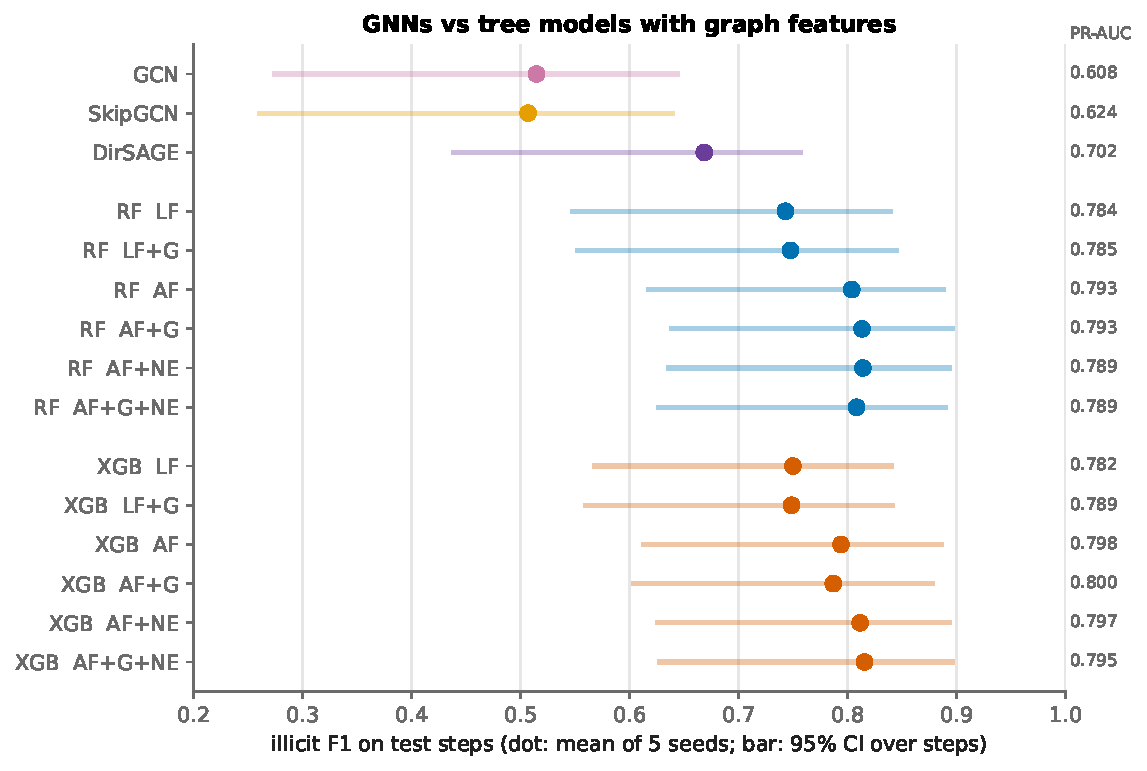
\includegraphics[width=\columnwidth]{../reports/figures/e04_graph.pdf}
  \caption{Illicit F1 of the graph neural networks and of the tree models on
  each feature set, with 95\% block-bootstrap intervals. Right: PR-AUC. LF local,
  AF all features, G structural graph features, NE GCN node embeddings.}
  \label{fig:graph}
\end{figure}
